%!TEX root = foo-thesis.tex

\chapter{Concept}
\label{chap:concept}

In this chapter, the presented global illumination system is explained on a conceptual level. After providing an overview of the rendering pipeline in the next section, the chosen approaches for the different components required for global illumination are outlined. Implementation details are deferred to the next chapter.

\section{Global Illumination Pipeline Overview}
\label{sec:concept:overview}

\begin{figure}[h]
    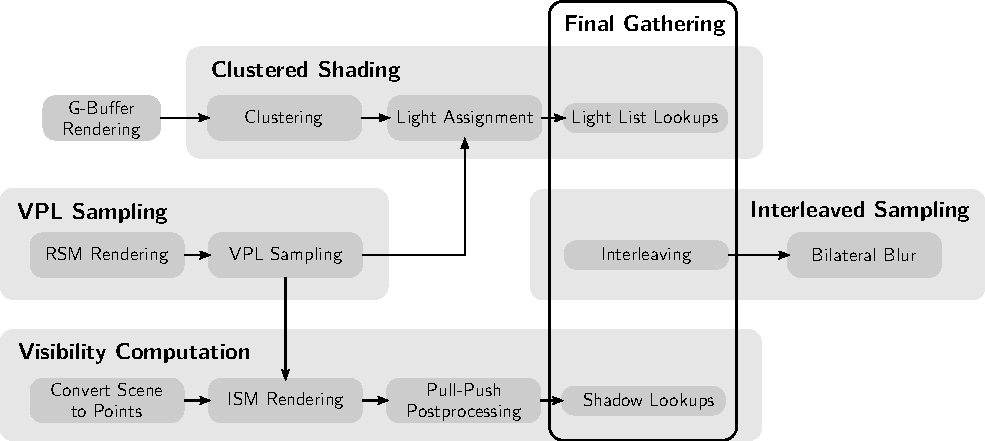
\includegraphics[width=\textwidth]{graphics/GI_pipeline_concept}
    \caption{The global illumination pipeline presented in this thesis.}
    \label{fig:GIPipelineConcept}
\end{figure}

\todo{ mention parts of final gathering somewhere in the text/caption}


\Cref{fig:GIPipelineConcept} provides an overview of the global illumination pipeline presented in this thesis.
Rendering the reflective shadow map and the subsequent VPL sampling (center row left in the diagram) will be covered in the following section.
\Cref{sec:concept:ism} describes the rendering process for imperfect shadow maps (lower row) in detail.
The final gathering step uses data from the clustered shading technique (upper row, detailed in \Cref{sec:concept:clusteredShading}) and performs interleaved sampling (right part of middle row, detailed in \Cref{sec:concept:interleavedSampling}).

During final gathering, clamping is used to remove singularities. Since this is a fairly trivial solution, it is not covered further.
In addition, the G-buffer rendering does not differ from common deferred rendering pipelines \citep{Saito:1990:ComprehensibleRendering} and is not covered further as well.


\section{Virtual Point Light Sampling with Reflective Shadow Maps}
\label{sec:concept:rsmVplSampling}

\begin{figure}[htb]
\centering
    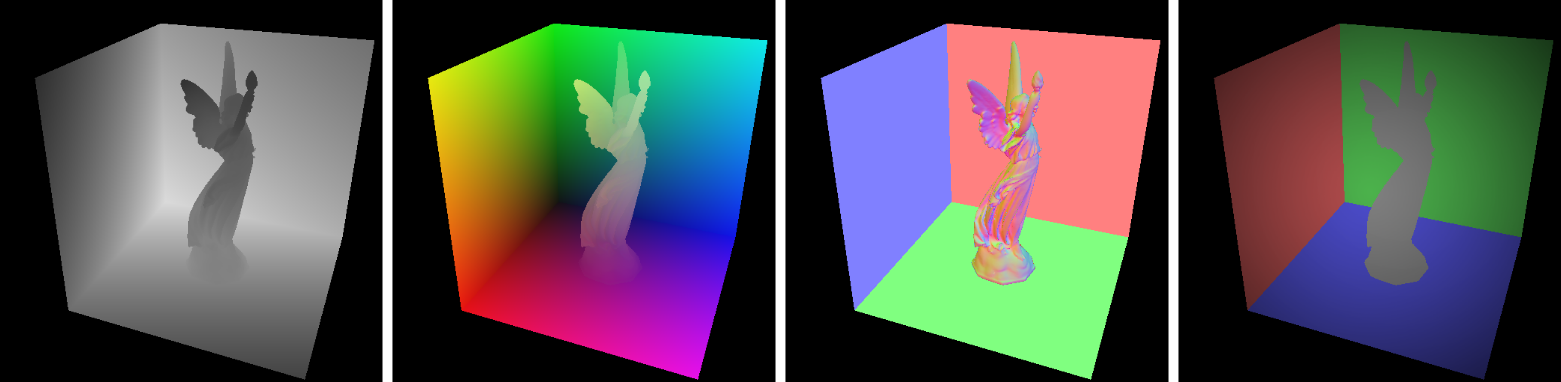
\includegraphics[width=\textwidth]{graphics/rsm_dachsbacher}
  \caption{A reflective shadow map as proposed by \citet{Dachsbacher:2005:RSM}. The buffers contain, from left to right, depth, world position, normal, and flux as a measure for light intensity. The flux buffer is used to account for different light intensities due to different solid angles of the pixels when using spot lights, and is not needed for directional lights. Figure reprinted from \citet{Dachsbacher:2005:RSM}.}
  \label{fig:concept:rsm_dachsbacher}
\end{figure}

Reflective shadow maps are often preferred as basis for VPL sampling techniques due to their simplicity and efficiency. Both of these advantages come from the fact that they are generated similar to conventional shadow maps, making them easy to implement and a perfect fit for GPUs. A downside is that they are well-suited only for computing the first light bounce.

Just like conventional shadow maps, RSMs render the scene from the viewpoint of a light. Besides the depth buffer used for shadow mapping, they render additional surface information, namely normal and color. As becomes apparent in \Cref{fig:concept:rsm_dachsbacher}, this is similar to the additional G-buffers created by conventional deferred rendering pipelines. The result can be sampled to create VPLs with a certain position reconstructed from the depth buffer, and normal and color taken from the additional buffers.

VPL sampling has not been the focus of this thesis, therefore we use a rather basic approach by creating an RSM and sampling it with a regular pattern. More advanced approaches are available (\Cref{sec:intro:relatedWorkManyLight:vplSampling}), some of which do not use RSMs (e.\,g., \cite{hedman2016sequential})


\section{Visibility Computation with Imperfect Shadow Maps}
\label{sec:concept:ism}

The original paper \citep{ritschel2008ism} converts the scene geometry to a point set in a preprocessing step and uses the points to efficiently render hundreds of shadow maps in parallel. For performance reasons, they use only a small subset of all points per shadow map, relying on the large number of shadow maps, each using a different subset, to keep the overall error small (\Cref{fig:concept:ism_ritschel_08}). They use splatting to render the points into shadow maps and fill the resulting holes with a simplified version of the pull-push algorithm presented by \citet{Marroquim:2007:reconstruction}. The technique is also capable of multi-bounce indirect illumination, which we have not implemented yet.

\begin{figure}[htb]
\centering
    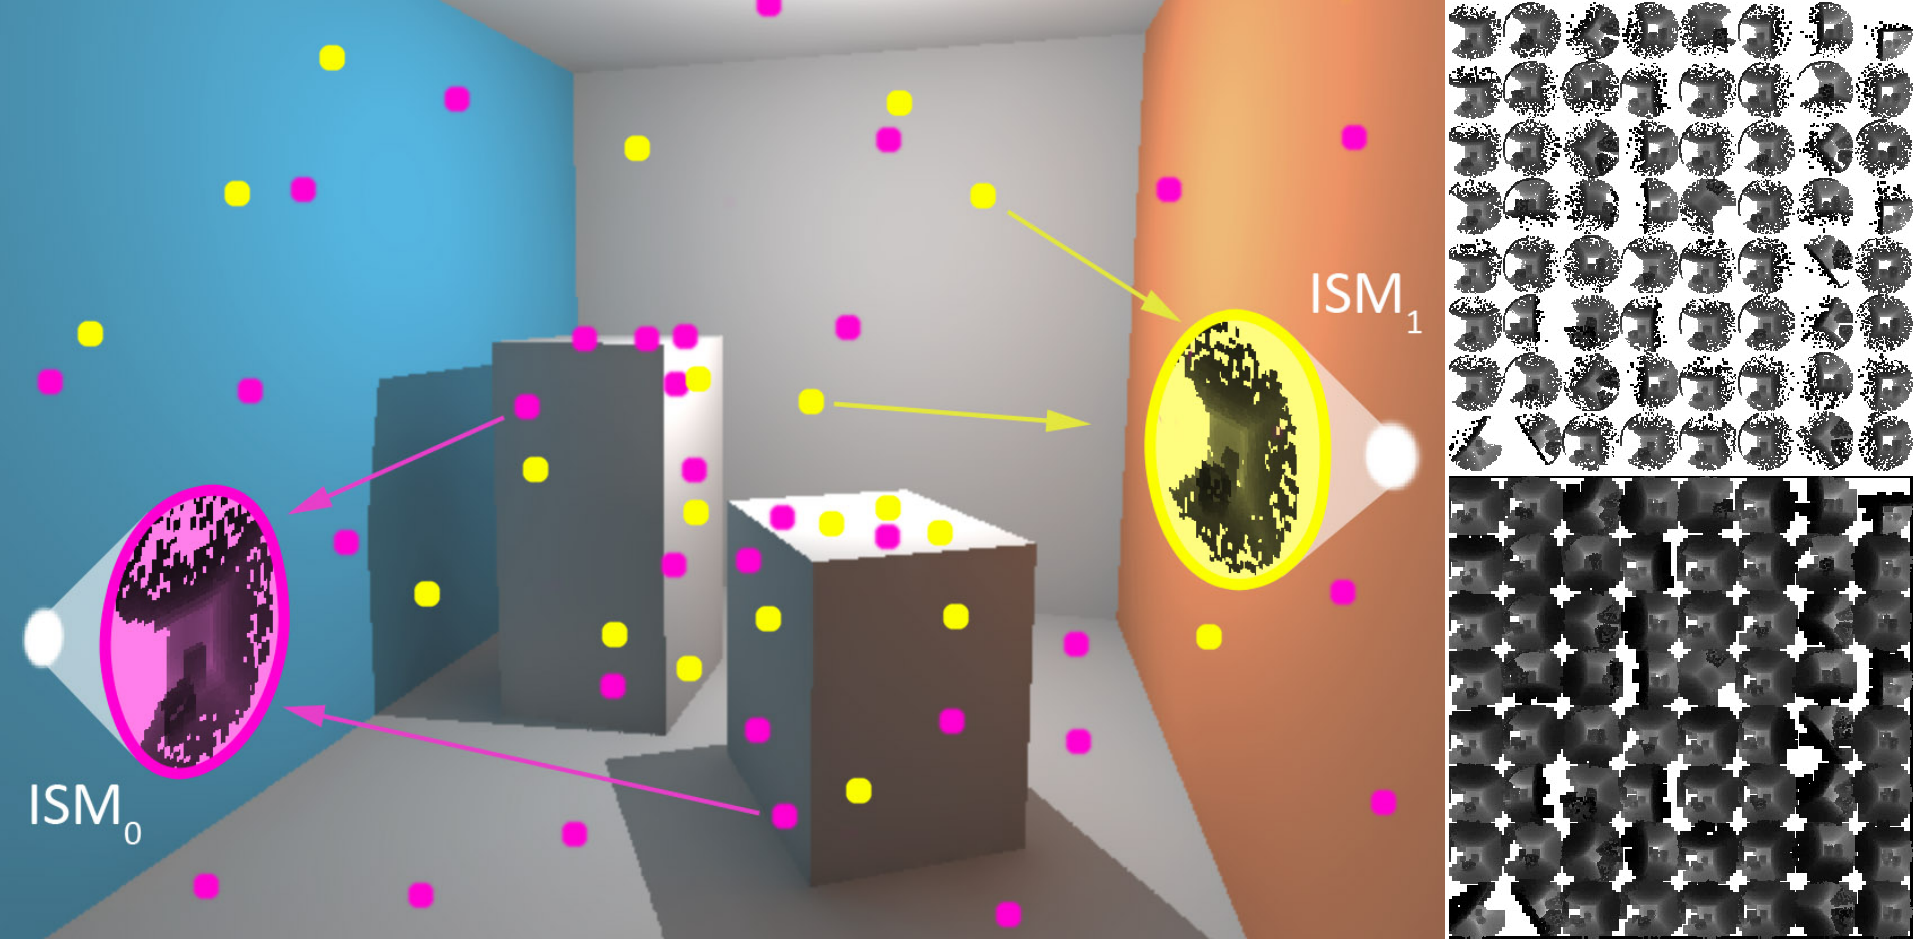
\includegraphics[width=\textwidth]{graphics/ism_ritschel_08}
  \caption{Illustration of imperfect shadow maps. For each VPL, a different set of points, colored yellow and pink, representing the scene is chosen. These are rendered into one small shadowmap per VPL (top right). A pull-push postprocessing algorithm fills holes in the shadowmaps (bottom right). Figure reprinted from \citet{ritschel2008ism}.}
  \label{fig:concept:ism_ritschel_08}
\end{figure}

\citet{ritschel2011ismsViewAdaptive} build on this by converting the scene to a triangle texture dynamically, and sampling the points from that texture. Instead of computing a triangle texture, \citet{barak2013temporally} use the tessellation units of recent GPUs to dynamically convert triangles into points.
We follow this approach since it integrates well into conventional rendering pipelines and by design supports dynamic geometry.

In contrast to \citet{ritschel2008ism}, we have found the pull-push postprocessing to be of little benefit when using regular point splatting. Instead, we demonstrate it shows its potential when used on single-pixel ``splats'' as proposed in the original paper. Additionally, rendering points as single pixels opens interesting optimization opportunities.

The following subsections describe the regular point splat rendering process and subsequently detail the pull-push algorithm that is used when rendering single-pixel points.


\subsection{Point Rendering with Splatting}

To convert the scene into points, all its triangles are first tessellated to meet a certain maximum size in order for the point conversion to not introduce extreme inaccuracies. Of the smaller tessellated triangles, the center and area are calculated and a point with matching center and area is created. While it might be more performant to create points just on the vertices of the triangles, at the same time it will be more inaccurate since this approach will enlarge the rendered area considerably over the triangle's extents.

Now a random VPL is chosen per point and backface culling is performed. Likewise, points that do not lie on the VPL's illuminated side are culled before splatting the point into the respective ISM. For performance reasons, a simple paraboloid projection is used for the ISMs in lieu of conventional cubemaps. Here, another advantage of using points comes into play: Compared to triangles, it is trivial to perform a paraboloid projection on them.

To remove holes in the resulting shadow map, \citet{ritschel2008ism} implement a simplified variant of \citet{Marroquim:2007:reconstruction} that only uses depth information from the point rendering. We found that this approach has little benefit over simply enlarging all the point splats during rendering, therefore we did not use it when using splat rendering.



\subsection{Point Rendering with Pull-Push Postprocessing}

As an alternative to point splat rendering, this subsection proposes a second approach that follows the algorithm of \citet{Marroquim:2007:reconstruction} more closely with the intent to obtain higher-quality shadow maps. More specifically, the points are rendered as a single pixel, albeit with additional attributes like size and normal. These are then used in a subsequent reconstruction pass to create an (ideally) hole-free shadow map (\Cref{fig:concept:pull_push_dataflow_marroquim}). This approach also allows a point to be rendered into multiple shadow maps with a moderate performance impact, more on this in \Cref{sec:impl:singlePixelRendering}.


\begin{figure}[htb]
\centering
    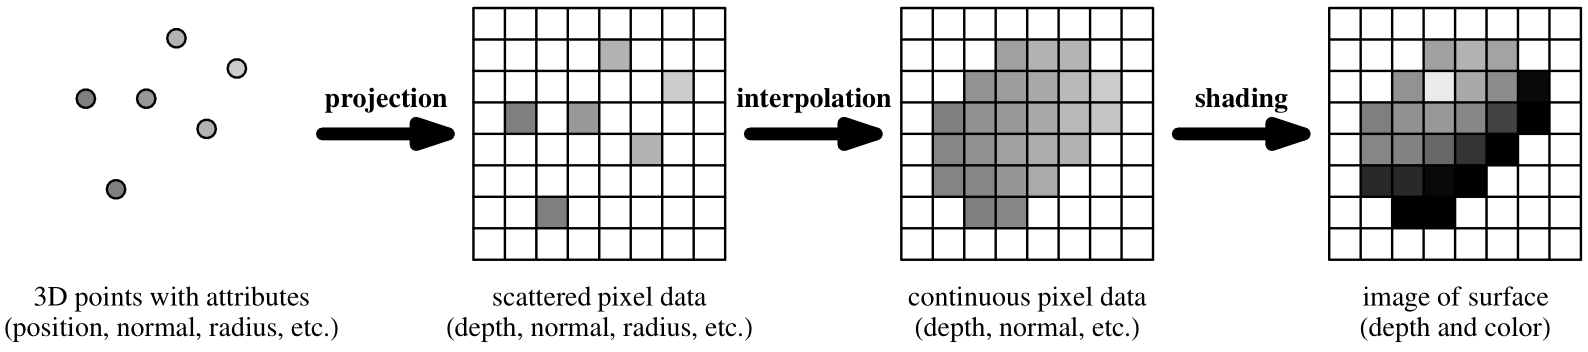
\includegraphics[width=\textwidth]{graphics/pullpush_dataflow_marroquim}
  \caption{Data flow of the pull-push surface reconstruction algorithm. Note that the shading step is skipped for rendering ISMs, as the depth information is sufficient. Figure reprinted from \citet{Marroquim:2007:reconstruction}.}
  \label{fig:concept:pull_push_dataflow_marroquim}
\end{figure}


To provide a rough overview, the pull-push algorithm proposed by \citet{Marroquim:2007:reconstruction} is a ``pyramid-method'' (\cite{Strengert:2006:Pyramid}) that uses the mipmap levels of a texture to first condense and then spread the data in the texture, in this case the sparse point set representing the scene. During the pull phase, it aggregates the information from four pixels of a finer level to one pixel of a coarser level. The subsequent push phase aggregates four pixels of a coarser level to one pixel of a finer level, but only if the pixel of the finer level contains no data or is determined to belong to an occluded surface. This way, closed surfaces are derived from single-pixel points.


\subsubsection{Pull Phase}
The pull phase reads four pixels of a finer level, computes an aggregate representation of them and writes the result to one pixel of the next coarser level. However, it only considers pixels that pass the following tests: First, they need to contain a valid depth at all (i.\,e., a point must have been rendered into this pixel) and second, the point in this pixel must not be occluded. A point is considered to be occluded if it is outside the depth interval of the frontmost of the four pixels used for interpolation.

Figuratively speaking, the depth interval of a point denotes the range in which other points are considered to belong to the same surface and can be used for interpolation. For the rendered points, the depth interval is simply $[d;d+k]$ where $d$ is the points depth and $k$ is a constant manually chosen to provide ``good'' results. For interpolated points, the new depth interval spans the interpolated depth of the point to the highest depth value of the depth intervals of all ``parent'' points.

To calculate the attributes for a new point, the depth and radius of the parent points are interpolated in between with equal weights (\Cref{fig:concept:weights_marroquim} (a) and (b)). Since the center of the aggregated point might not match the position of the pixel (this happens if not all four pixels are used for interpolation), a displacement vector is also calculated and stored to accurately describe the point's location.

\begin{figure}[htb]
  \centering
  \begin{subfigure}[b]{0.25\textwidth}
    \centering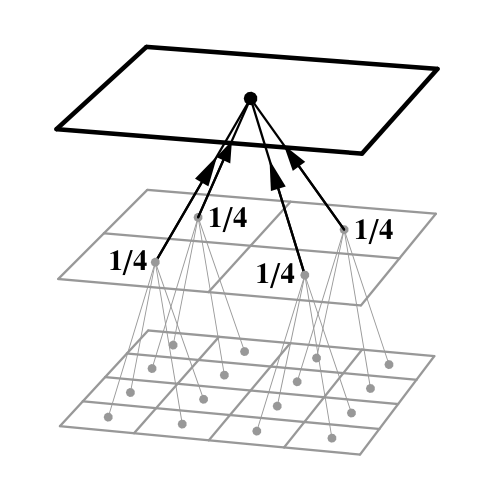
\includegraphics[width=\textwidth]{graphics/pull_weights_marroquim1}
    \caption{}
  \end{subfigure}%
  \begin{subfigure}[b]{0.25\textwidth}
    \centering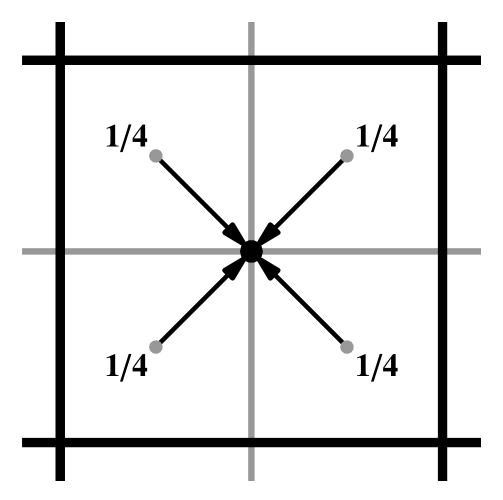
\includegraphics[width=\textwidth]{graphics/pull_weights_marroquim2}
    \caption{}
  \end{subfigure}%
  \begin{subfigure}[b]{0.25\textwidth}
    \centering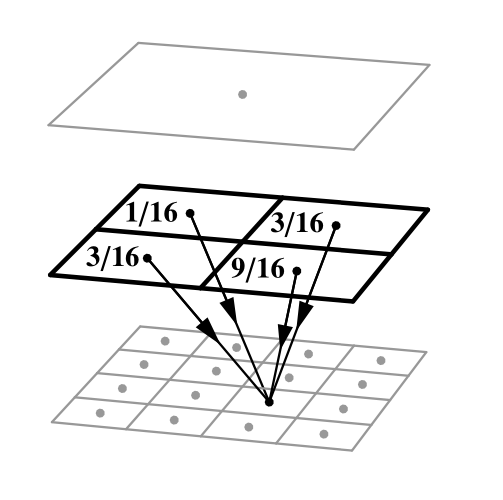
\includegraphics[width=\textwidth]{graphics/push_weights_marroquim1}
    \caption{}
  \end{subfigure}%
  \begin{subfigure}[b]{0.25\textwidth}
    \centering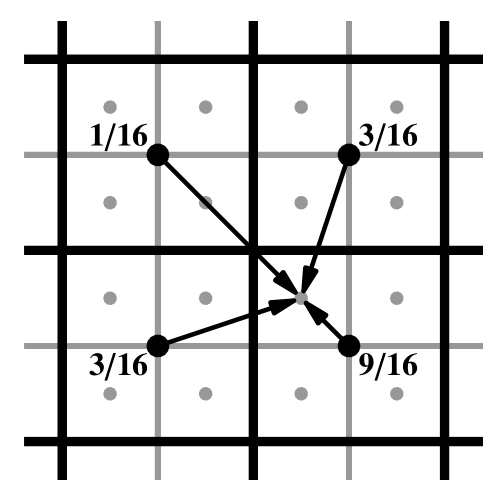
\includegraphics[width=\textwidth]{graphics/push_weights_marroquim2}
    \caption{}
  \end{subfigure}
  \caption{Illustration of the weights used for interpolation during the pull phase ((a) and (b)) and push phase ((c) and (d)). Figures reprinted from \citet{Marroquim:2007:reconstruction}.}
  \label{fig:concept:weights_marroquim}
\end{figure}



\subsubsection{Push Phase}

Analogous to the pull phase, the push phase reads four pixels of the coarser level, rejects pixels that do not pass certain tests, and writes one output pixel into the finer level. First, just like in the pull phase, the input pixels must contain a valid depth and not be occluded to be considered. Additionally, a radius check is performed: If the pixel's location is outside the point's extents described by the displacement vector and its radius, then the point is not considered either. This is done to limit a point's influence to its actual size.

The target output location in the finer level might already contain data that was computed during the pull phase. This data is overwritten if its depth is behind the interpolated point's depth interval, i.\,e., if the original data is considered to be occluded. Otherwise, the original point is left untouched, as it is likely more accurate than the previously computed, interpolated point.

Since the input and output pixel's location do not match the way they do during the pull phase, the weights used for interpolation during the push phase are not uniform (\Cref{fig:concept:weights_marroquim} (c) and (d)).

 \citet{Marroquim:2007:reconstruction} also use each point's normal to correctly limit the point's size, and \citet{Marroquim:2008:reconstruction2} propose Gaussian weights based on the pixel's distance to the point's location, instead of constant weights solely based on pixel locations. Both of these additions we have not implemented yet.



 \section{Interleaved Sampling}
 \label{sec:concept:interleavedSampling}
 Interleaved sampling \citep{Keller:2001:InterleavedSampling} is often used to tremendously improve the performance of GI methods with a negligible quality impact. The general idea is as follows: Instead of calculating all samples per pixel, the samples are distributed over a block of pixels. Now, since each pixel processes only part of all samples, there is obviously information missing per pixel. Visually, this becomes apparent in the form of structured noise. To this end, a bilateral blur that preserves geometry edges similar to \citet{laine2007incremental} is used to spread the information and thereby even out the noise. The blur is often implemented in a separated fashion for performance reasons, although strictly speaking, bilateral filters are not separable.

 Since adjacent pixels now access disjoint sets of samples, naive implementations of this technique usually show bad cache coherence. To improve on this, \citet{segovia2006non} proposed \textit{non-interleaved shading of interleaved sample patterns}, or for short \textit{de-interleaving}. They group those pixels that use the same sample set into smaller sub-buffers, coherently process each buffer, and then merge the sub-buffers to one large buffer again. See \Cref{fig:concept:interleaved_segovia} for the intermediate results of this algorithm.


 \begin{figure}[htb]
     \centering
     \begin{subfigure}[b]{0.33\textwidth}
         \centering
         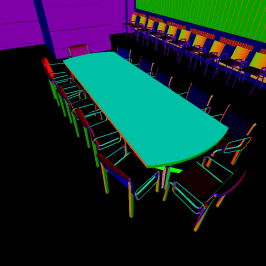
\includegraphics[width=0.95\textwidth]{graphics/interleaved_segovia_1}
         \caption{}
         \label{fig:concept:interleaved_segovia_1}
         \end{subfigure}%
         \begin{subfigure}[b]{0.33\textwidth}
             \centering
             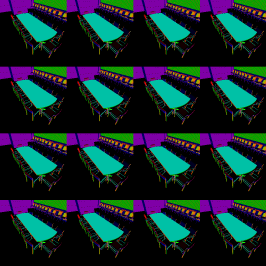
\includegraphics[width=0.95\textwidth]{graphics/interleaved_segovia_2}
             \caption{}
             \label{fig:concept:interleaved_segovia_2}
             \end{subfigure}%
             \begin{subfigure}[b]{0.33\textwidth}
                 \centering
                 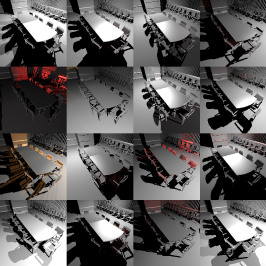
\includegraphics[width=0.95\textwidth]{graphics/interleaved_segovia_3}
                 \caption{}
                 \label{fig:concept:interleaved_segovia_3}
             \end{subfigure}
             \begin{subfigure}[b]{0.33\textwidth}
                 \centering
                 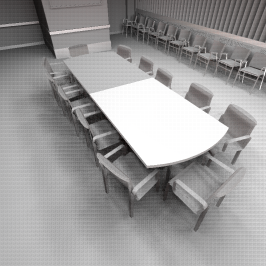
\includegraphics[width=0.95\textwidth]{graphics/interleaved_segovia_4}
                 \caption{}
                 \label{fig:concept:interleaved_segovia_4}
                 \end{subfigure}%
                 \begin{subfigure}[b]{0.33\textwidth}
                     \centering
                     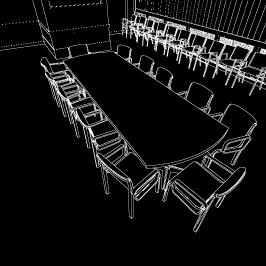
\includegraphics[width=0.95\textwidth]{graphics/interleaved_segovia_5}
                     \caption{}
                     \label{fig:concept:interleaved_segovia_5}
                     \end{subfigure}%
                     \begin{subfigure}[b]{0.33\textwidth}
                         \centering
                         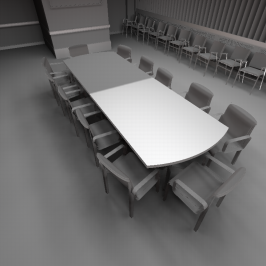
\includegraphics[width=0.95\textwidth]{graphics/interleaved_segovia_6}
                         \caption{}
                         \label{fig:concept:interleaved_segovia_6}
                     \end{subfigure}
                     \caption{Visualization of the de-interleaving process. (a) The original G-buffer. (b) The G-buffer is split into multiple smaller sub-buffers. (c) Each sub-buffer is processed using a different set of lights. (d) The sub-buffers are re-interleaved to one large buffer. (e) A depth discontinuity buffer is computed for the next step. This is usually omitted in modern implementations. (f) A bilateral blur is applied to mask the noise visible in (d). Figures reprinted from \citet{segovia2006non}.}
                     \label{fig:concept:interleaved_segovia}
                 \end{figure}


                 Effectively, when applied to blocks of $n^2$ pixels, this technique cuts down the cost of sampling by $ 1 / n^2 $ at the expense of smoothing high-frequency changes in the samples over $n$ pixels. Since global illumination is usually of low frequency, i.\,e., adjacent pixels usually receive a similar amount of indirect light, interleaved sampling does not significantly affect quality when applied to global illumination. However, this approach falls short near depth and normal discontinuities, where the bilateral blur has to ignore several pixels. Nevertheless, even in this case the quality degradation is hardly noticeable as soon as the global illumination results are blended over the rendered image (\Cref{sec:results:interleavedShading}).

                 In most aspects we follow the standard approach for interleaved sampling. The only notable deviation is the implementation of de-interleaving that does not use any separate splitting and merging passes. For details, see \Cref{sec:impl:interleavedShading}.



\section{Clustered Deferred Shading}
\label{sec:concept:clusteredShading}

In real-time graphics applications, primarily video games, a technique called \textit{clustered shading} \citep{olsson2012clustered}, has seen increased usage. Its goal is to increase the efficiency of lighting a scene with multiple light sources.
The effectiveness of clustered shading in the context of many-light global illumination has not been studied so far to our knowledge, and this thesis aims to contribute a few data points to this end.

The clustered shading technique works as follows: First, the view frustum is divided into a fixed number of three-dimensional clusters. For each fragment, the respective cluster is determined with the purpose of ignoring all clusters with no fragments in them. Then, each cluster is ``assigned'' a list of all lights that potentially illuminate fragments in that cluster, i.\,e., whose illuminated region is intersecting with a bounding volume of the cluster (\Cref{fig:concept:clustered_olsson}). All lights not intersecting a cluster are culled, i.\,e., not added to the cluster's light list.

\begin{figure}[htb]
\centering
    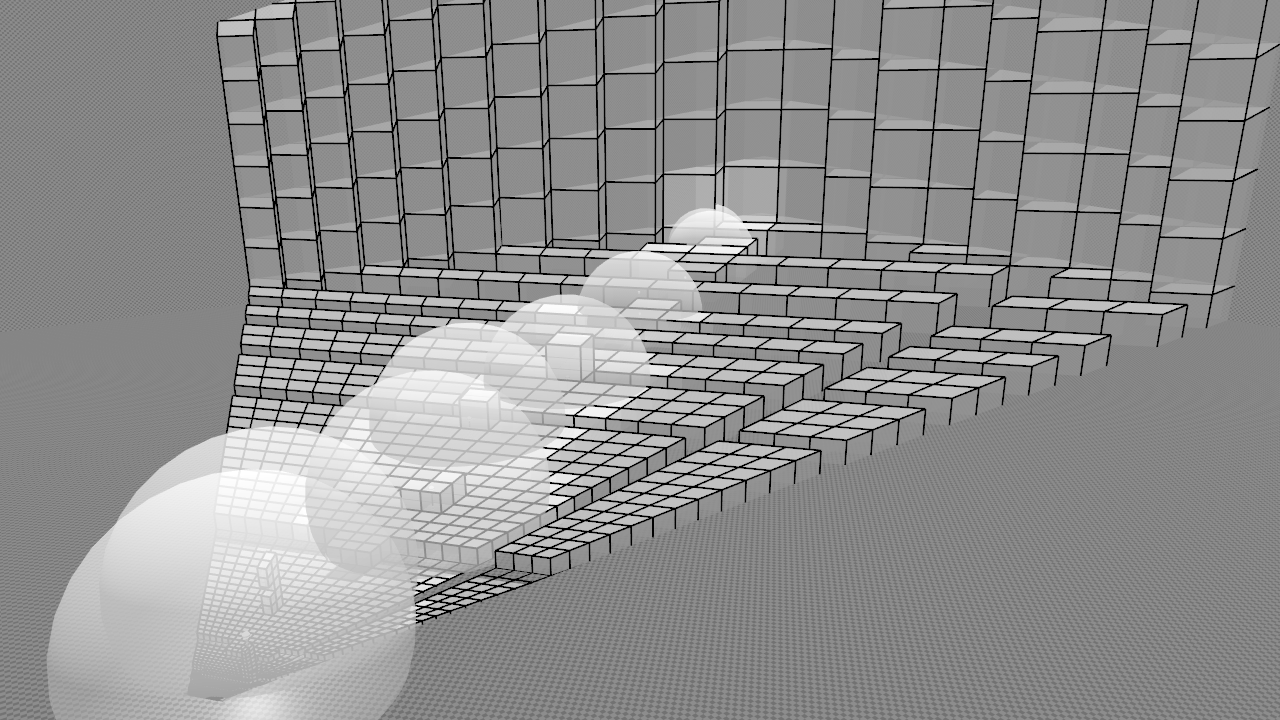
\includegraphics[width=\textwidth]{graphics/clustered_olsson}
  \caption{Visualization of clusters (cubes) and light ranges (spheres) used for the light assignment step. Each cluster is assigned a list of all lights whose influence spheres are intersecting the cluster. Figure reprinted from \citet{Olsson:2015:manylightmanagement}.}
  \label{fig:concept:clustered_olsson}
\end{figure}


When shading a fragment, the algorithm first determines the fragment's cluster again, and then iterates only over the lights in that cluster's light list. This way, all the lights that have been discarded in the previous step do not need to be considered per fragment.

This technique yields the most gains when using lights with a limited radius. In that case, the culling is all the more effective since all lights that are farther away from a cluster than the light's radius can be culled as well. However, many-light methods often use infinite radii to enable light transport over long distances. Nonetheless, one can still expect to cull roughly half of all lights with this technique in a many-light context, since VPLs have a field of view of 180° instead of being completely spherical.

As an extension, \citet{olsson2012clustered} propose to calculate explicit bounds for the fragment's position in each cluster to enable more precise culling. We expected only moderate performance gains from that and have not implemented it. Another possible extension is to use the surface normal's direction as fourth dimension after the three spatial dimensions for clustering, allowing for a kind of backface culling for even greater efficiency.


Clustered shading is an extension and improvement to \textit{tiled shading} \citep{Olsson:2011:TiledShading}, which uses screen-space tiles instead of three-dimensional view-space clusters. Tiled shading has previously been combined with many-light global illumination by \citet{Tokuyoshi:2016:Stochastic}. They use an order of magnitude more lights than we do, but stochastically limit them in range. As a result, the light culling is much more effective in their case.
We implemented tiled shading as well and will compare it to clustered shading in \Cref{sec:results:clusteredShading}.
